\section{Database}
\label{sec:database}

A database is an important part of any system which is designed to provide a
mechanism for storing, managing and retrieving information. PostgreSQL, an
object-relational database, was considered for the project. The two reasons
behind choosing PostgreSQL were---availability on School's system and
familiarity with the database model. The database designer considered business
rules and processes during requirements analysis and came up with an initial
draft of database model. The model was reviewed with the team and some
modifications were done to accommodate the system requirements. The server used
to create database was dbteach2. A new database, called osakagp, was created to
store the data needed for Edify quiz.

\subsection{Tables}
\label{sub:tables}

The four tables created in osakagp DB are \verb+quiz+, \verb+questions+,
\verb+users+ and \verb+users_result+.

\begin{description}

	\item[\texttt{Users}] \hfill \\ The user login details are stored in the
		users table. The user details are inserted into this table when a new
		user or Admin registers. The login credentials entered by the users are
		validated and the users are allowed to login only if the entered
		credentials exist in the users table.

	\item[\texttt{Quiz}] \hfill \\ The quiz topics are stored in this table.
		The quiz could be on the following topics---Politics, Sports, History,
		Geography, Music, and Science and Technology. The Admin chooses the
		quiz topic from quiz table and fetches the topic-related questions from
		the questions table.

	\item[\texttt{Questions}] \hfill \\ The questions table contains the
		questions which are answered in quiz. Question and possible answers
		are stored as rows in the questions table. The table also contains a
		separate column for quiz ID\@. The Admin uses the quiz ID to get the
		questions for the chosen quiz topic.

	\item[\texttt{User\_result}] \hfill \\ This table contains the quiz results
		for all the Students. It is loaded with quiz result once the quiz is
		completed. The user can see the result by quiz date, quiz topic, score
		and quiz status.

\end{description}

\subsection{Entity-Relationship Diagram}
\label{sub:entity_relationship_diagram}

\begin{figure}[htpb]
	\centering
	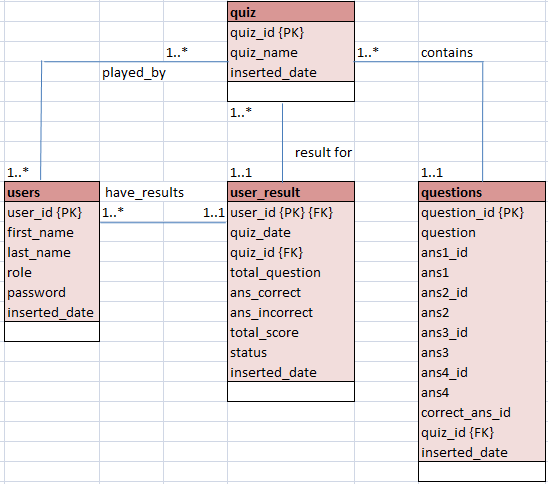
\includegraphics[width=0.8\linewidth]{img/Entity_Relationship_Diagram.png}
	\caption{This is the entity-relationship (ER) diagram for the tables used
	in Edify quiz. The relationship shared among these tables is explained in
	Section~\ref{sub:entity_relationship_diagram}.
	}\label{fig:entity_relationship_diagram}
\end{figure}

\subsubsection{One-to-one}
\label{ssub:One-to-one}
\begin{itemize}

	\item The table questions shares a one-to-one relationship with quiz table.
		Each question in the questions table can appear only in one quiz
		category.

	\item The table \verb+user_result+ shares a one-to-one relationship with
		users and quiz tables.The \verb+user_result+ table stores the result of
		all the quizes played by the Students. Each row in the
		\verb+user_result+ table is linked to one quiz in the quiz table and
		one user in the users table.

	\item The \verb+user_result+ table shares one-to-one relationship with
		users table. Each row in the \verb+user_result+ table is linked to one
		user in the users table.

\end{itemize}

\subsubsection{One-to-Many}
\label{ssub:One-to-Many}

\begin{itemize}

	\item The quiz table shares one-to-many relationship with questions table.
		Each quiz topic has 10 questions in the questions table.

	\item The quiz table shares one-to-many relationship with
		\verb+users_result+ table. Each quiz topic in the quiz table is linked
		to multiple rows in the \verb+users_result+ table as quiz result is
		stored for multiple players and can be played on multiple days.

	\item The quiz table shares one-to-many relationship with users table. One
		quiz can be played by mutilple users in the users table.

	\item The users table shares one-to-many relationship with quiz table. Each
		user in the users table can play one or more quiz in the quiz table.

	\item The users table shares one-to-many relationship with
		\verb+user_result+ table. Each user in the users table can have one or
		more quiz results in the \verb+user_result+ table.

\end{itemize}

\subsection{Normalization}
\label{sub:normalization}

Data normalization was implemented to reduce and eliminate data redundancy.

\begin{description}

	\item[First Normal Form] \hfill \\ All the tables are in 1NF as they
		contain only atomic values and there are no repeating groups of data.

	\item[Second Normal Form] \hfill \\ All tables are in 1NF and all of their
		non-key attributes are fully dependent on their primary keys. There is
		no partial dependency of any column on primary key.

	\item[Third Normal Form] \hfill \\ All the tables are in 1NF and 2NF and
		all non-key attributes are fully functional dependent only on the
		primary key.

\end{description}
